\chapter{Audio Data Reception}

\label{AudioDataReception}

The system is versatile and is capable of handling a wide variety of input audio data streams. The scope of this work, 
however, focuses on the reception of web browser audio input and \ac{voip} audio input.

%----------------------------------------------------------------------------------------

\section{Audio Connection}

Any specific audio reception point returns the generic AudioConnection class and allows the rest of the system to 
handle every audio connection the same. It contains data about its assigned session, the user it belongs to, and the 
audio input channel it uses.

It also provides an event-based interface so the rest of the system can listen to specific events and react  
accordingly. The available events are the "close" event, which gets fired when the audio connection gets closed, and 
the "message" event, which gets fired when new data from the audio stream is available.

This architecture provides a unified interface for the entire system to handle audio streams and their data.

\begin{verbatim}
// audioConnection.ts
export type EventType = "message" | "close";
export class AudioConnection {
    get closed() {}
    readonly id: string;
    readonly sessionId: string;
    readonly userId: string;
    readonly userName: string | undefined;
    readonly rtpRegisterEntry: RTPRegisterEntry | undefined;

    constructor(
        id: string,
        sessionId: string,
        userId?: string,
        userName?: string,
        rtpRegisterEntry?: RTPRegisterEntry,
    ) {}

    emitMessage(message: Buffer) {}
    close() {}
    on(type: EventType, cb: (arg: Buffer | void) => void): number {}
    off(id: number) {}
}
\end{verbatim}

%----------------------------------------------------------------------------------------

\section{Web Browser Audio}

The web browser audio input is the most straightforward audio input channel. It is based on WebSockets and
uses the WebSocket \ac{api} to receive audio data from the client. The client uses the MediaRecorder \ac{api} to 
capture the audio data from the microphone and sends it to the server via the WebSocket connection.

\subsection{Transmitter}

The web browser joins a WebSocket connection to the server and sends the audio data as a binary message to the server. 
It requests access to the microphone and uses the MediaRecorder API to capture the audio data. 
The audio data is requested in chunks of approximately 200ms and sent to the server as a \ac{webm}-encoded binary 
message.

\subsection{Receiver}

On the other hand, the receiving WebSocket Server takes the chunk, converts the data into a \ac{wav} file format by 
utilizing \cite{ffmpeg2023}, and fires the appropriate AudioConnection "message" event to inform all listeners about 
the new data.

%----------------------------------------------------------------------------------------

\section{Voice-over-IP Audio}

The \ac{voip} audio input is more complicated than the WebSocket solution for the web browser. It is based on \ac{udp} 
for the audio stream and requires additional \ac{http} \ac{api} endpoints to register incoming streams properly.

\subsection{Transmitter}

The transmitting side of the \ac{voip} audio input is the \ac{voip} provider. Third parties implement it, and its 
detailed implementation is out of the scope of this work. The \ac{voip} provider sends the audio data as a \ac{udp} 
stream to the system with approximately 20ms of audio data per chunk. Each chunk contains an identifier that allows the 
system to map the audio data to a specific user. For the system to identify the audio data and assign it to the correct 
connections and sessions, the \ac{voip} provider registers the audio stream via an \ac{http} \ac{api} endpoint like the 
one shown below.

\begin{verbatim}
POST /api/v1/register-rtp
{
    "ssrcId": 87C12C,
    "callbackPort": 35200,
    "sessionId": "22265aba-f96b-55b2-8335-5a19cf757096",
    "userId": "e96249a4-ae55-5120-b51b-b57401b29955",
}
\end{verbatim}

The \textbf{ssrcId} property is the unique identifier for the \ac{udp} stream. The \textbf{callbackPort} property is 
the system's port to send \ac{udp} messages to the \ac{voip} provider. The \textbf{sessionId} and \textbf{userId} 
properties are the identifiers for the session and user to whom the audio stream belongs.

\subsection{Receiver}

The receiving side of the \ac{voip} audio input is the system. It receives the \ac{udp} stream from the \ac{voip} 
provider. It concatenates the chunks to a complete audio stream by utilizing the \textbf{ssrcId} property and 
cross-referencing it with the registered streams. Since this is already a \ac{wav} audio stream, the system can 
directly fire the appropriate AudioConnection "message" event to inform all listeners about the new data.

\subsection{Communication Flow}

In the diagram below \ref{fig:voip-communication-flow}, the communication flow between the \ac{voip} provider and the 
System is shown (in this graphic called "Alternis"). It shows the registration via the \ac{http} \ac{api} endpoint and 
the continuous \ac{udp} stream of audio data. The \ac{voip} provider sends the audio data to the System, and the System 
sends the translated audio data back to the \ac{voip} provider. 

\begin{figure}[ht]
	\centering
	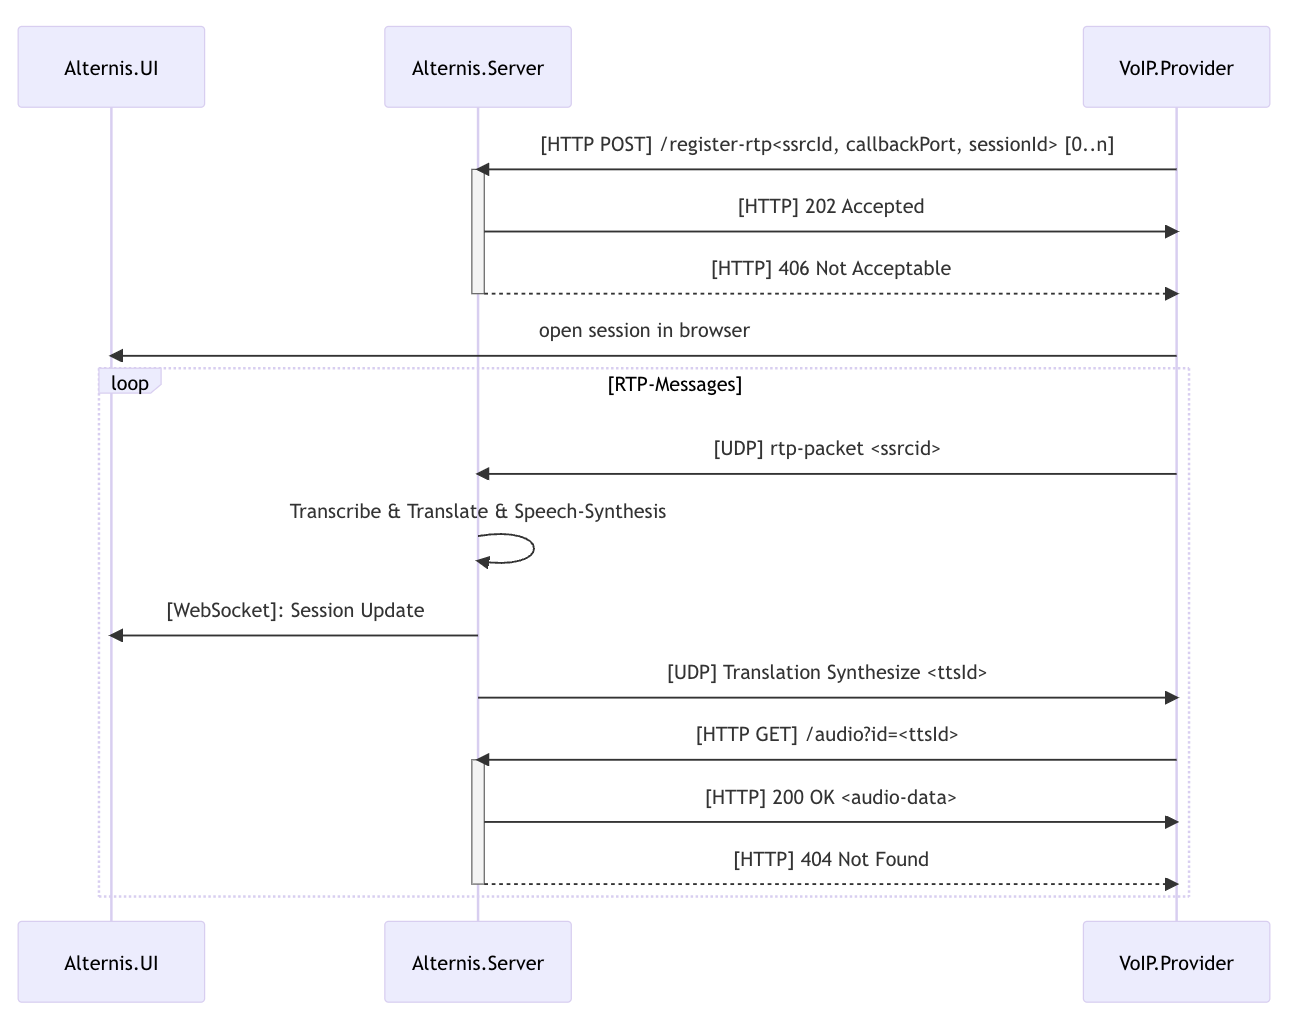
\includegraphics[width=0.8\textwidth]{Figures/voip-communication-flow.png}
	\caption{VoIP Communication Flow}
	\label{fig:voip-communication-flow}
\end{figure}
